\documentclass[
	%sans,			% use sans-serif font
	%serif,			% use serif-font
	%mathsans,		% set mathtext to sans-serif
	%mathserif,		% set mathtext to serif
	%10pt,
	10pt,
	%12pt,
	t		% add text at the top border of slide
	%slidescentered,% center text on slide
	%draft,			% compile as draft version
	%handout,		% create handout file
	%notes,			% include nodes in slides
	%compress		% compress navigation bar
]{beamer}

\usetheme{lmtslides}
\usepackage{eso-pic}
\usepackage{graphicx}
%\usepackage[pdftex]{color}
\usepackage{times}
\usepackage[latin1]{inputenc}
%\usepackage[T1]{fontenc}
\usepackage[amssymb]{SIunits}
\usepackage{amsmath,amssymb}
\usepackage{eurosym}
\usepackage{booktabs}
\usepackage{colortbl}
\usepackage{url}
\usepackage[absolute,overlay]{textpos}
\usepackage{graphicx}
\usepackage{mathtools}

\renewcommand{\footnoterule}{\vfill\kern -3pt  \kern 2.6pt}

\setbeamertemplate{caption}{\raggedright\insertcaption\par}
\setbeamertemplate{bibliography item}[online]
\graphicspath{{figures/}}

\setlang{en}		

% Supervisor: Univ.-Prof. Dr. Hans-Joachim Bungartz
% Advisors: Manish Kumar Mishra, M.Sc. (hons) &
% Samuel James Newcome, M.Sc.

% MODIFY THESE ACCORDINGLY! ---
\title{Exploring Fuzzy Tuning Technique for Molecular Dynamics Simulations in AutoPas}
\type{Bf} % (M/B/D/S)(f/m): (Master/Bachelor/Diplom/Studienarbeit)(final/midterm)
\author{Manuel Lerchner}
\email{manuel.lerchner@tum.de}
\advisorOne{Manish Kumar Mishra, M.Sc. (hons)}
\advisorTwo{Samuel James Newcome, M.Sc.}
\date{\today}
%------------------------------


%%%%%%%%%%%%%%%%%%%%%%%%%%
\begin{document}

\maketitle


\section{AutoPas}
\begin{frame}
	\frametitle{What is AutoPas?}

	\begin{textblock*}{5cm}(9cm,1.8cm)
		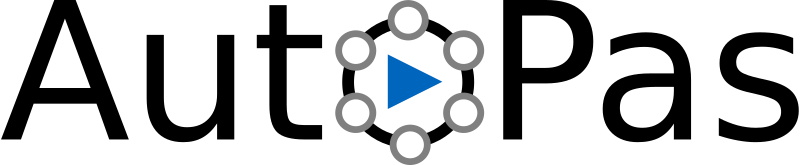
\includegraphics[width=3cm]{figures/AutoPasLogo}
	\end{textblock*}


	\begin{itemize}
		\item Library for optimal node-level performance in N-body simulations
		\item Many different implementations for the N-body problem
		\item AutoTuning: Automatically switch between implementations
		      \begin{itemize}
			      \item \textbf{Container:} How to find neighboring particles?
			      \item \textbf{Traversal:} How to handle multi-threading?
			      \item \textbf{Data Layout:} How to store particles in memory?
			      \item \textbf{Newton 3:} Can we exploit Newton's 3rd law?
			      \item \dots
		      \end{itemize}
		\item Example applications:
		      \begin{itemize}
			      \item \texttt{md\_flexible} (Molecular Dynamics)
			      \item \texttt{sph} (Smoothed Particle Hydrodynamics)
		      \end{itemize}
	\end{itemize}
\end{frame}


\begin{frame}
	\frametitle{Structure of AutoPas}

	\begin{itemize}
		\item Three main components:
		      \begin{itemize}
			      \item User Application
			      \item Algorithm Library
			      \item Tuning Strategies
		      \end{itemize}
		\item Algorithm Library:
		      \begin{itemize}
			      \item Huge Search Space\footnote{\scriptsize{$\text{Container}\times\text{Traversal} \times \text{Data Layout} \times \text{Newton 3} \times \text{Load Estimator} \times \text{Cell Size Factor}$}
			            }
		      \end{itemize}
		\item Tuning Strategies:
		      \begin{itemize}
			      \item Full Search
			      \item Random Search
			      \item Predictive Tuning
			      \item Bayesian Search
			      \item Rule Based Tuning
		      \end{itemize}
	\end{itemize}

	\begin{textblock*}{4cm}(8cm,2cm)
		\begin{figure}
			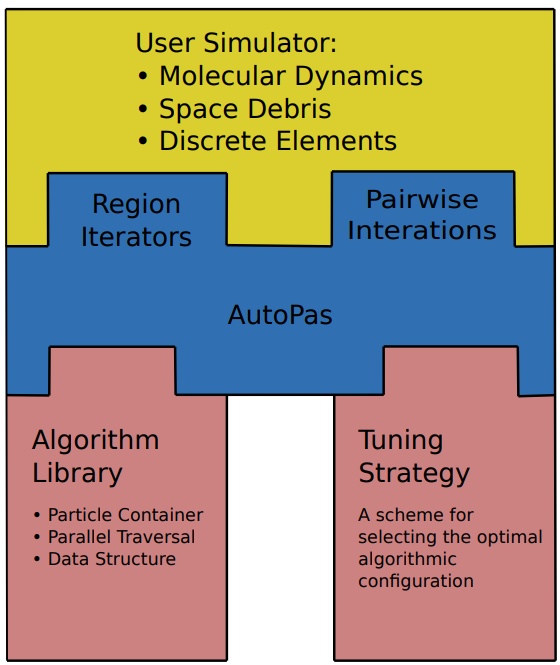
\includegraphics[width=4cm]{figures/AutoPasLibraryStructure.png}
			\caption{ \footnotesize{Source: \cite{Newcome2023Poster}}}

		\end{figure}
	\end{textblock*}
\end{frame}



\begin{frame}
	\frametitle{Auto-Tuning }

	\begin{itemize}
		\item Tuning Phase: Find the best configuration
		      \begin{itemize}
			      \item Tuning Strategies select configurations to evaluate
			      \item Expensive, Time consuming
		      \end{itemize}
		\item Simulation Phase: Use the best configuration
	\end{itemize}

	\vspace{0.2cm}

	\begin{center}
		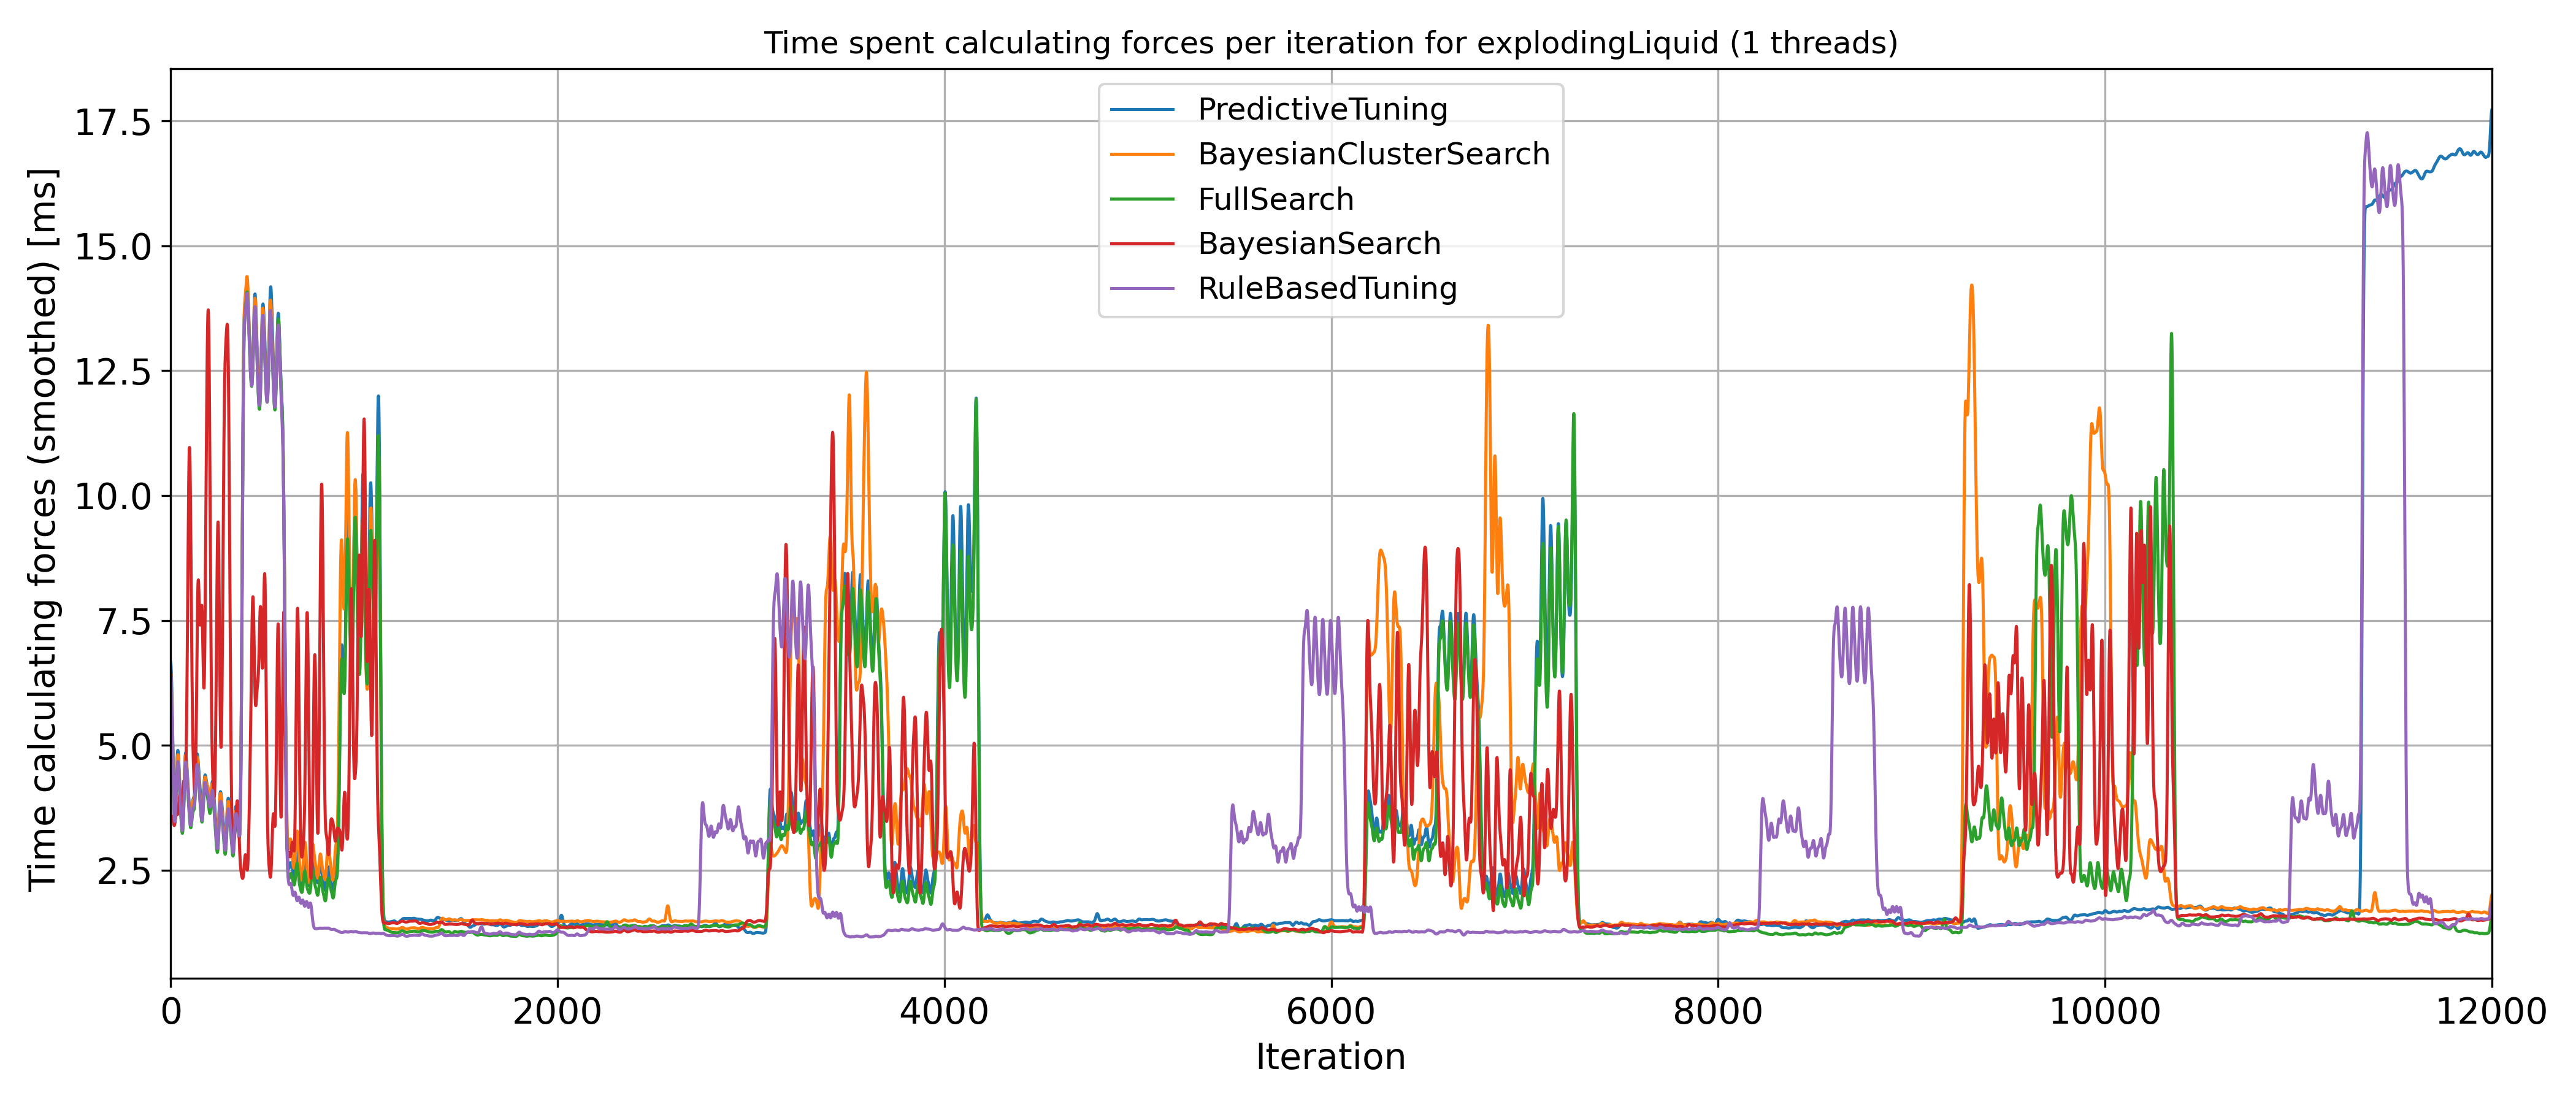
\includegraphics[width=0.95\textwidth,trim={0 0 0 0.85cm},clip]{figures/timing_explodingLiquid.png}
	\end{center}


\end{frame}

\section{Fuzzy Logic}
\begin{frame}
	\frametitle{Fuzzy Logic Systems}

	\begin{itemize}
		\item Use human-like reasoning to model complex systems
		\item Example: Heater Control
		      \begin{itemize}
			      \item Input: temperature (e.g. 20$^{\circ}$C), humidity (e.g. 50\%)
			      \item Output: heater power (e.g. 50\%)
			      \item Rules:
			            \begin{tabular}{lcll}
				            \textbf{IF}  temp is \textit{cold} & \textbf{AND} & humidity is \textit{dry} & \textbf{THEN}  power is \textit{high}   \\
				            \textbf{IF}  temp is \textit{hot}  & \textbf{OR}  & humidity is \textit{wet} & \textbf{THEN}  power is \textit{low}    \\
				            \textbf{IF}  temp is \textit{warm} &              &                          & \textbf{THEN}  power is \textit{medium} \\
			            \end{tabular}
		      \end{itemize}
		\item Very easy to understand and interpret
		\item Can handle uncertainty and imprecise information
		\item Complexity is abstracted away in the linguistic terms (e.g. \textit{cold, warm, hot})
		\item Fuzzy System $f: \mathbb{R}^n \rightarrow \mathbb{R}$
	\end{itemize}

\end{frame}

\begin{frame}
	\frametitle{Mathematical Foundations}

	\begin{itemize}
		\item Consider the Fuzzy Rule:
		      \[
			      \underbrace{  \underbrace{\textbf{IF}  \;(\underbrace{\text{temp}}_{\text{Ling. Var.}} \text{is} \underbrace{\textit{cold}}_{\text{Ling. Term}}  \textbf{AND}  \underbrace{\text{hum}}_{\text{Ling. Var.}} \text{is} \underbrace{\textit{dry}}_{\text{Ling. Term}}) }_{\text{Antecedent}}
				      \textbf{THEN}  \underbrace{\underbrace{\text{power}}_{\text{Ling. Var.}} \text{is} \underbrace{\textit{high}}_{\text{Ling. Term}}}_{\text{Consequent}}
			      }_{\text{Fuzzy Rule}}
		      \]
		\item Fuzzy Logic Systems consist of:
		      \begin{itemize}
			      \item Linguistic Terms / Fuzzy Sets (e.g. \textit{cold, warm, hot})
			      \item Linguistic Variables (e.g. temperature, humidity, power)
			      \item Fuzzy Logic Operators (e.g. \textbf{AND, OR, NOT})
			      \item Fuzzy Rules (e.g. \textbf{IF} \textit{antecedent} \textbf{THEN} \textit{consequent})
		      \end{itemize}
	\end{itemize}
\end{frame}

\begin{frame}
	\frametitle{Fuzzy Sets}
	\begin{itemize}
		\item Fuzzy Sets are generalizations of classical sets
		      \begin{itemize}
			      \item Classical Sets: binary membership function $\in_A : A \rightarrow \{false, true\}$
		      \end{itemize}
		\item Fuzzy Sets are defined by:
		      \begin{itemize}
			      \item Underlying Crisp Set $X$ (e.g. $age \subseteq \mathbb{R}$)
			      \item \textbf{Continuous} membership function $\mu_{\tilde{A}} : X  \rightarrow [0,1]$
		      \end{itemize}
		\item Allow for uncertainty. When is a person young?
	\end{itemize}
	\begin{center}
		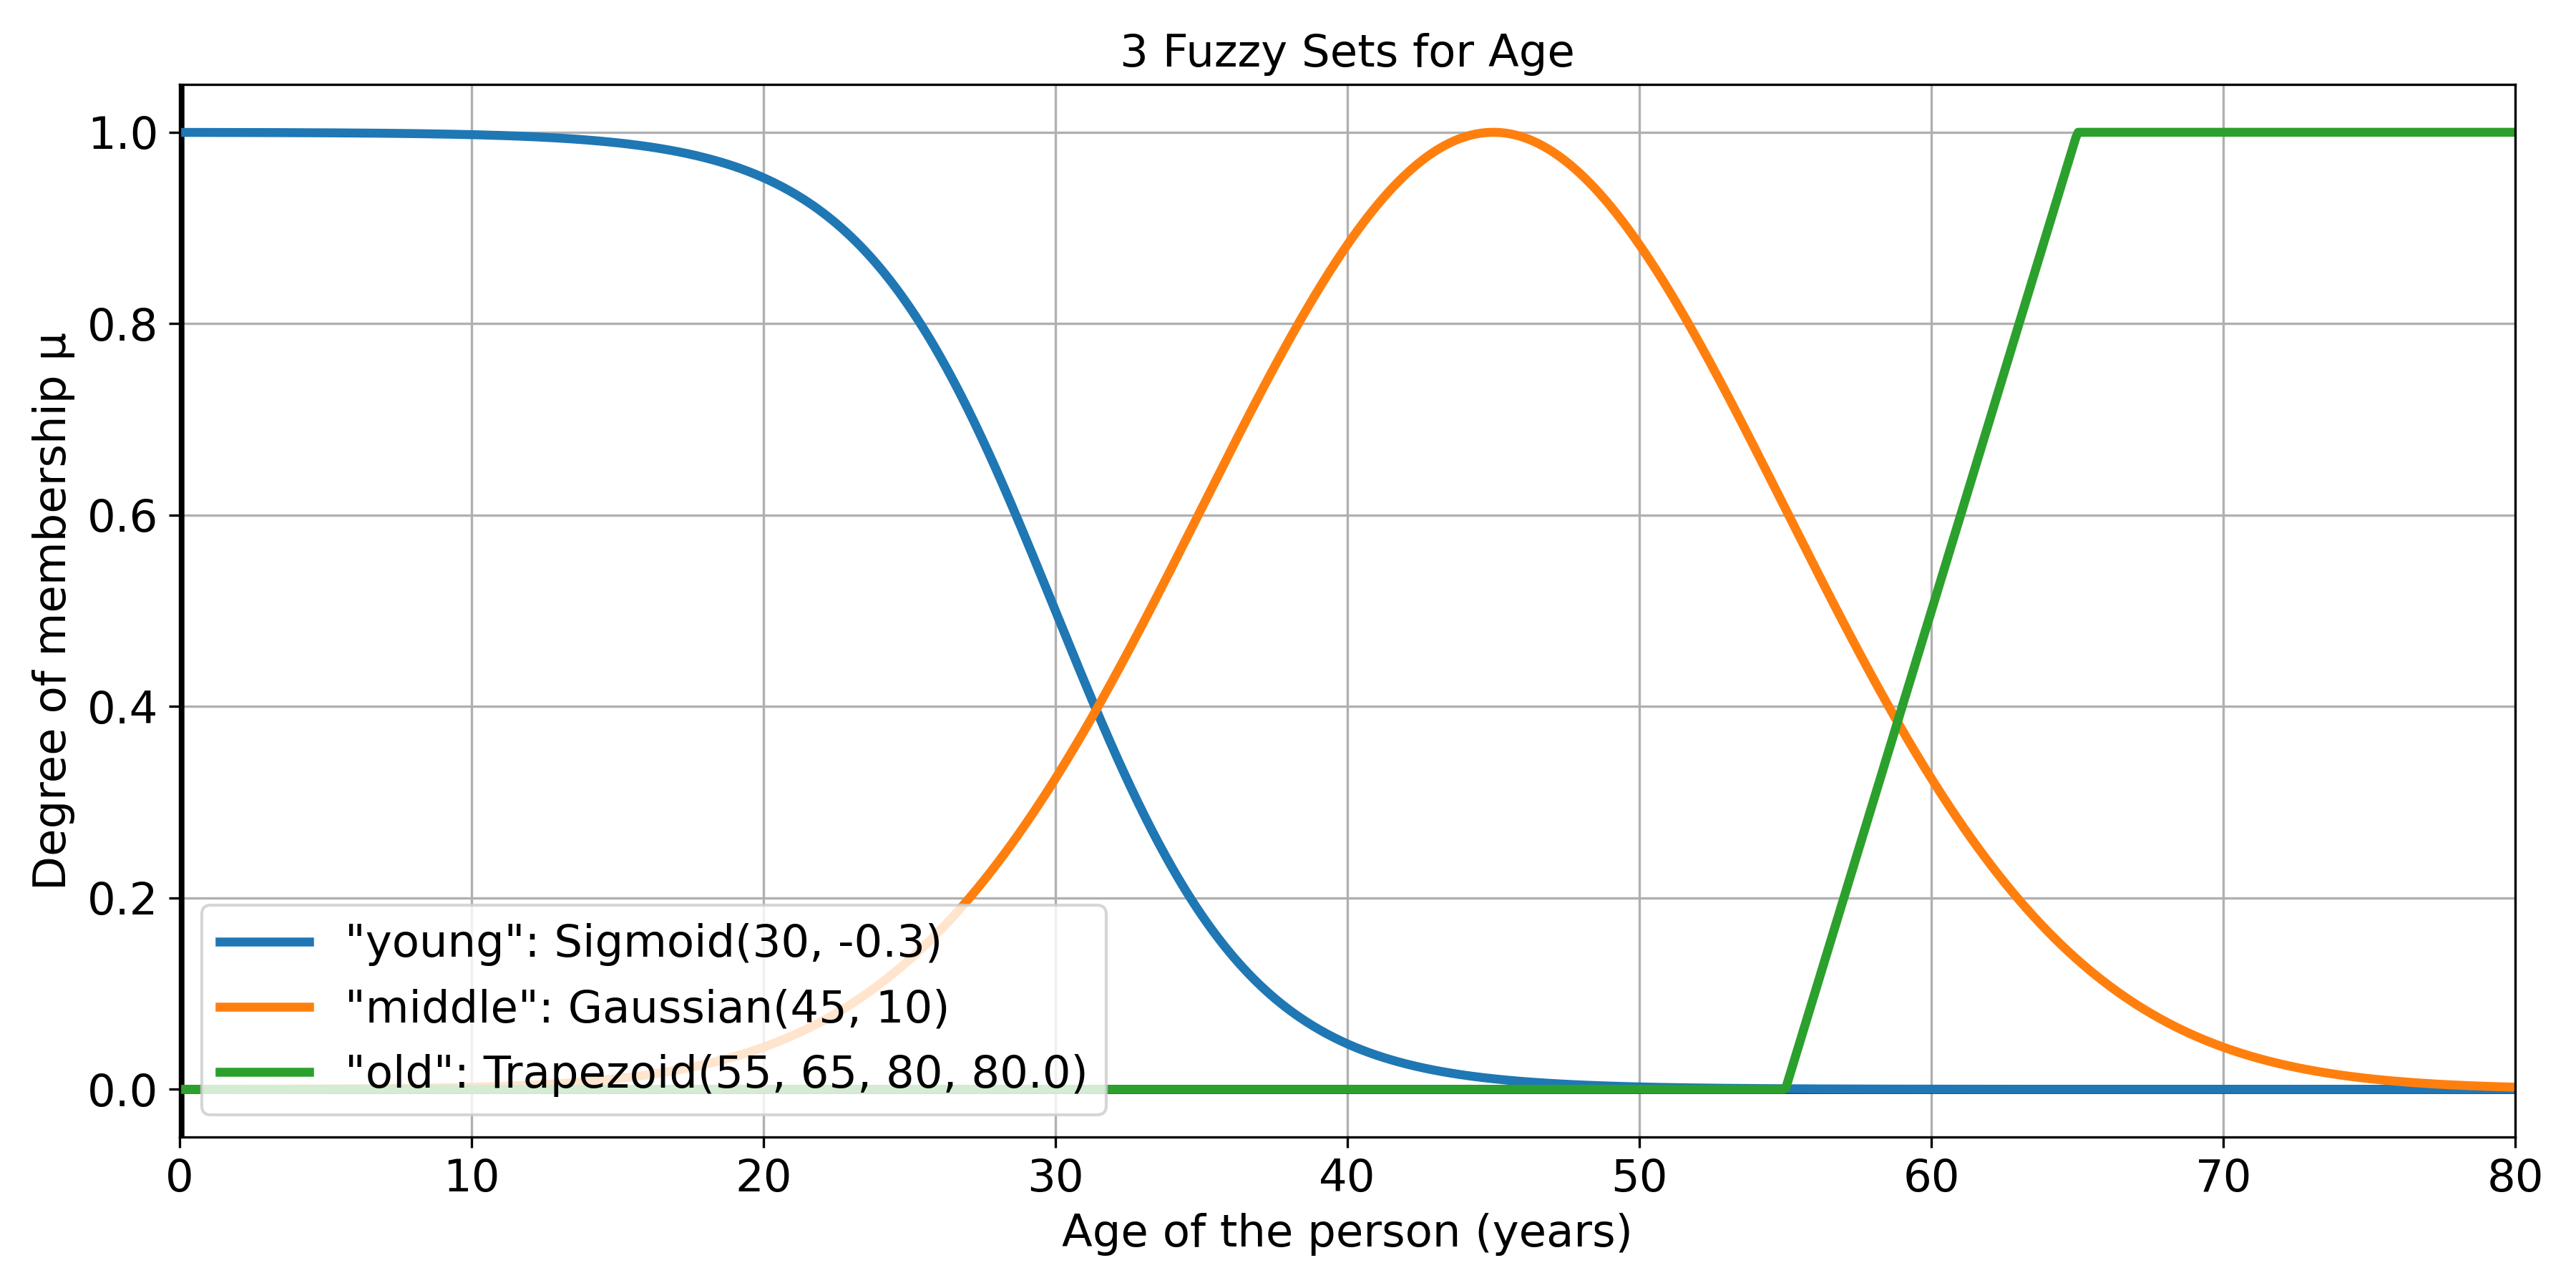
\includegraphics[width=0.75\textwidth,trim={0 0 0 0.85cm},clip]{figures/age-fuzzy-sets.png}
	\end{center}
\end{frame}

\begin{frame}
	\frametitle{Linguistic Variables}
	\begin{itemize}
		\item Linguistic Variables can take on linguistic terms / fuzzy sets
		      \begin{itemize}
			      \item E.g. \textit{age} can take \textit{young}, \textit{middle-aged} or \textit{old}
		      \end{itemize}
		\item Instead of using crisp values (35 years), we use a combination of linguistic terms to describe the age (Fuzzyification):
		      \[ \text{ 35 years} \implies  \begin{cases}
				      \text{20\% young}       \\
				      \text{60\% middle-aged} \\
				      \text{0\% old}
			      \end{cases}
		      \]
		\item This allows for non-numerical reasoning:
		      \begin{itemize}
			      \item E.g. \textbf{IF} age is \textit{young} \textbf{THEN} fitness is \textit{high}
			      \item Use abstract concepts instead of crisp values
		      \end{itemize}
		\item Each linguistic term represents a certain \textit{collection} of values
	\end{itemize}
\end{frame}

\begin{frame}
	\frametitle{Fuzzy Logic Operators}
	\begin{itemize}
		\item Fuzzy Logic Operators are used to modify/combine fuzzy sets
		\item Extension of boolean logic operators to real numbers
		      \begin{itemize}
			      \item $\wedge : \{false, true\} \times \{false, true\} \rightarrow \{false, true\}$
			      \item $\textbf{AND} : [0,1] \times [0,1] \rightarrow [0,1]$
		      \end{itemize}
		\item Extended operators need to maintain the classical semantics
		\item Typically, Fuzzy Logic Operators are defined as:
		      \begin{itemize}
			      \item \textbf{AND:} Corresponds to the intersection of fuzzy sets
			            \[ \mu_{\tilde{A} \cap \tilde{B}}(x) = \min(\mu_{\tilde{A}}(x), \mu_{\tilde{B}}(x)) \]
			      \item \textbf{OR:} Corresponds to the union of fuzzy sets
			            \[ \mu_{\tilde{A} \cup \tilde{B}}(x) = \max(\mu_{\tilde{A}}(x), \mu_{\tilde{B}}(x)) \]
			      \item \textbf{NOT:} Corresponds to the complement of a fuzzy set
			            \[ \mu_{\neg \tilde{A}}(x) = 1 - \mu_{\tilde{A}}(x) \]

		      \end{itemize}
	\end{itemize}
\end{frame}

\begin{frame}
	\vspace{0cm}
	\begin{figure}
		\centering
		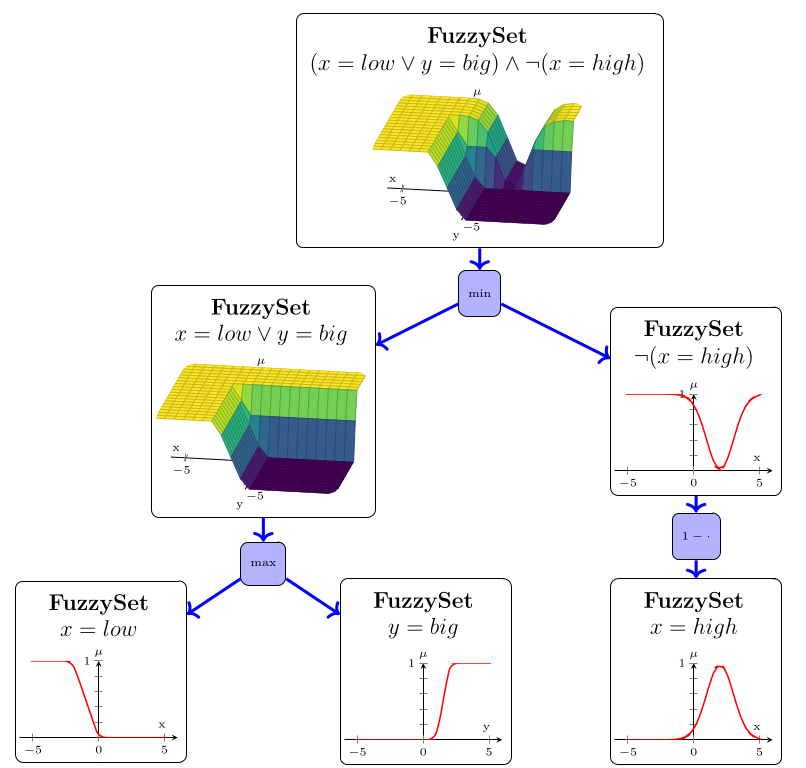
\includegraphics[height=0.62\paperwidth]{figures/RecursiveFuzzyTree.png}
	\end{figure}
\end{frame}

\begin{frame}
	\frametitle{Fuzzy Rules}
	\begin{itemize}
		\item Each rule is of the form: $\textbf{IF} \; {antecedent} \; \textbf{THEN} \; {consequent}$
		      \begin{itemize}
			      \item Both antecedent and consequent are fuzzy sets
			      \item E.g. $\textbf{IF} \; \text{age} \; \text{is} \; \textit{young} \; \textbf{THEN} \; \text{fitness} \; \text{is} \; \textit{high}$
		      \end{itemize}
		\item Rules can be interpreted as a logical implication
		      \begin{itemize}
			      \item $\textbf{IF} \; \tilde{A} \; \textbf{THEN} \; \tilde{B} \quad \iff \quad \tilde{A} \;  \textbf{IMPLIES} \;  \tilde{B}$
			      \item Implication is similar to previous operators (\textbf{AND, OR, NOT})
			      \item Special form of implication: Mamdani Implication
			            \begin{itemize}
				            \item $\tilde{R} = \textbf{IF} \; \tilde{A} \; \textbf{THEN} \; \tilde{B}$
				            \item $\mu_{\tilde{R}}(x) = \min(\mu_{\tilde{A}}(x), \mu_{\tilde{B}}(x))$
			            \end{itemize}
			      \item \textit{Effect} of the rule is limited by the \textit{strength} of the antecedent
		      \end{itemize}
		\item A Fuzzy System can consist of multiple rules acting on the same linguistic variable
		      \begin{itemize}
			      \item The total \textit{effect} on the output is the combination/union of all individual rule outputs
		      \end{itemize}
	\end{itemize}
\end{frame}

\begin{frame}
	\frametitle{Defuzzification}
	\begin{itemize}
		\item Process of converting arbitrary fuzzy sets to a crisp value
		      \begin{itemize}
			      \item Special case: Fuzzy sets resulting from rule application
			            \[  \begin{cases}
					            \text{20\% young}       \\
					            \text{60\% middle-aged} \\
					            \text{0\% old}
				            \end{cases} \implies \text{35 years}
			            \]
		      \end{itemize}
		\item Multiple methods for defuzzification:
		      \begin{itemize}
			      \item \textbf{Centroid:} Weighted average of the fuzzy set
			            \[ \text{Centroid} = \frac{\int x \cdot \mu_{\tilde{R}}(x) dx}{\int \mu_{\tilde{R}}(x) dx} \]
			      \item \textbf{Mean of Maxima:} Average of all maxima of the fuzzy set
		      \end{itemize}
		\item Core idea: Represent aspects of the fuzzy set with a crisp value
		      \begin{itemize}
			      \item E.g. Weighted average of all possible values (Centroid)
			      \item E.g. Most likely value (Mean of Maxima)
		      \end{itemize}
	\end{itemize}

\end{frame}



\begin{frame}
	\vspace{-0.8cm}
	\begin{figure}
		\centering
		\caption{\tiny{Source: \href{https://de.mathworks.com/help/fuzzy/fuzzy-inference-process.html}{MathWorks - Fuzzy Inference Process}}}
		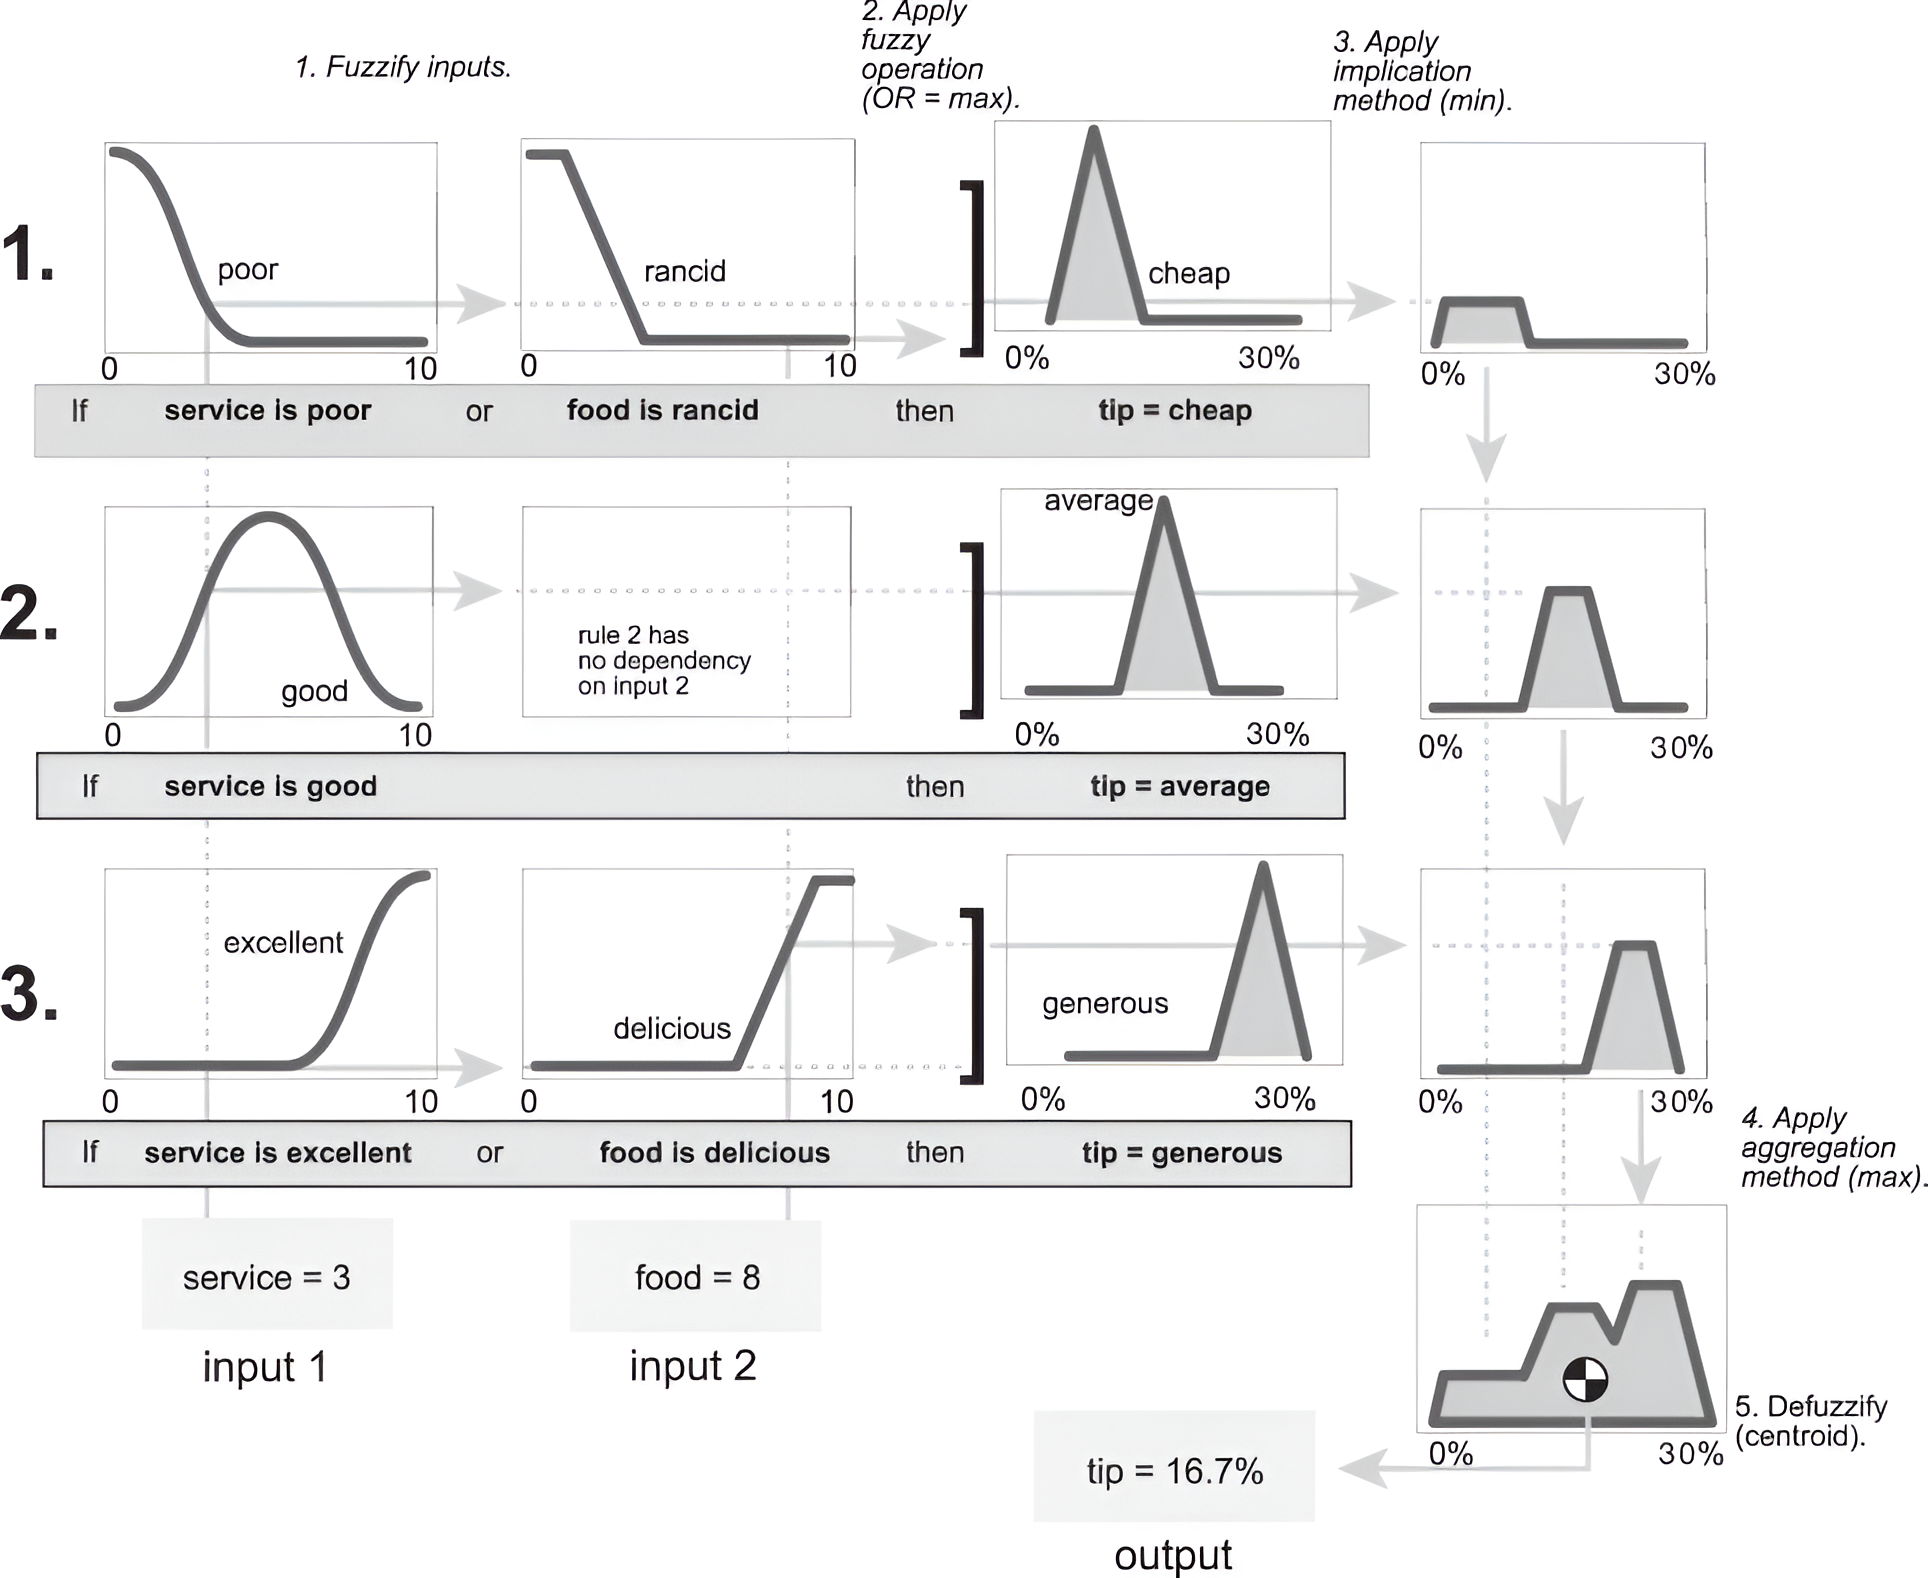
\includegraphics[width=0.8\paperwidth]{figures/FullInferenceProcess.png}
	\end{figure}
	\label{fig:fuzzy_inference_full}

\end{frame}


\begin{frame}
	\begin{itemize}
		\item TODO: Maybe add decision surfaces here
	\end{itemize}
\end{frame}

\section{Fuzzy Tuning Strategy}
\begin{frame}
	\frametitle{Fuzzy Tuning Strategy}

	\begin{itemize}
		\item Main Idea: Use Fuzzy Logic to tune AutoPas
		\item Make use of LiveInfoData\footnote{Simulation state: \texttt{avgParticles/Cell, homogeneity, threadCount \dots }} to perform tuning
		\item Benefits:
		      \begin{itemize}
			      \item Similar to Rule-Based Tuning
			      \item Potentially more expressive and powerful
			      \item Still easy to understand and interpret
		      \end{itemize}
		\item Challenges and Questions for AutoPas:
		      \begin{itemize}
			      \item What are the output variables? How to predict Configurations?
			      \item How to interpret the result? (Fuzzy System : $f :\mathbb{R}^n \rightarrow \mathbb{R}$ )
			      \item How to create the fuzzy rules? Expert knowledge?
			      \item How to specify the linguistic terms / fuzzy sets?
		      \end{itemize}
	\end{itemize}
\end{frame}

\section{Approaches}
\begin{frame}
	\frametitle{Approach 1: Component Tuning}
	\begin{itemize}
		\item Independently predict good values/patterns for each tunable parameter
		\item Create a Fuzzy System for each tunable parameter
		      \begin{itemize}
			      \item Container\_DataLayout
			      \item Traversal
			      \item Newton 3
		      \end{itemize}
		\item Output Variables: Nominal Representation of parameter values
		\item Numeric output mapped to the closest value {\footnotesize \cite{Mohammed2022}}
		\item Combine the patterns to obtain final configurations
	\end{itemize}

	\begin{figure}
		\centering
		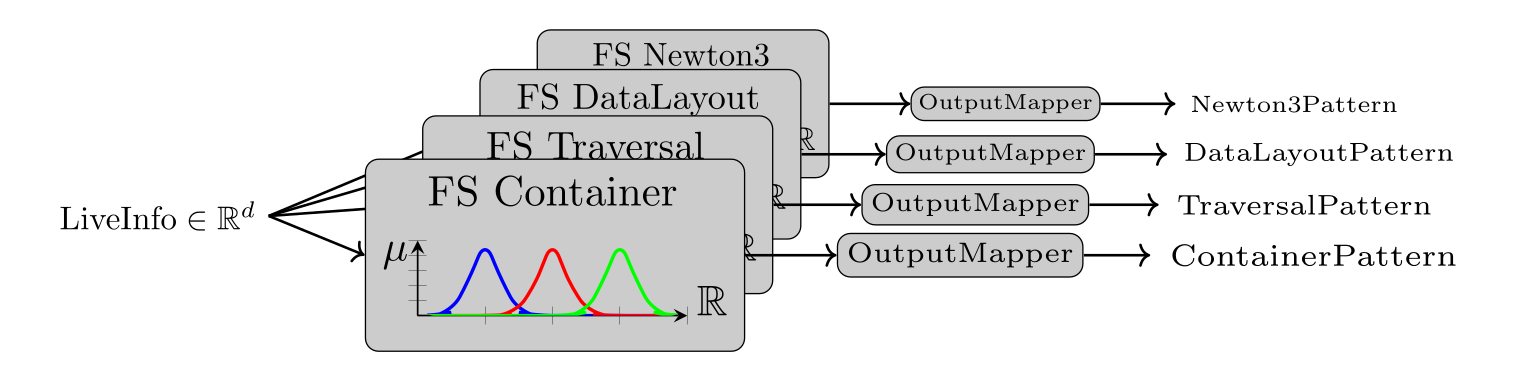
\includegraphics[width=1\textwidth]{figures/component-approach.png}
	\end{figure}

\end{frame}


\begin{frame}
	\frametitle{Approach 1: Component Tuning}
	\begin{itemize}
		\item TODO Linguistic Variables
	\end{itemize}

\end{frame}




\begin{frame}
	\frametitle{Approach 2: Suitability Tuning}
	\begin{itemize}
		\item Predict the suitability of \textit{each} configuration
		\item Use the suitability values to determine worthwhile configurations
		\item Create a Fuzzy System for each possible configuration
		\item Output Variables: Suitability of the configuration
		\item More complex, but potentially more powerful
	\end{itemize}

	\begin{figure}
		\centering
		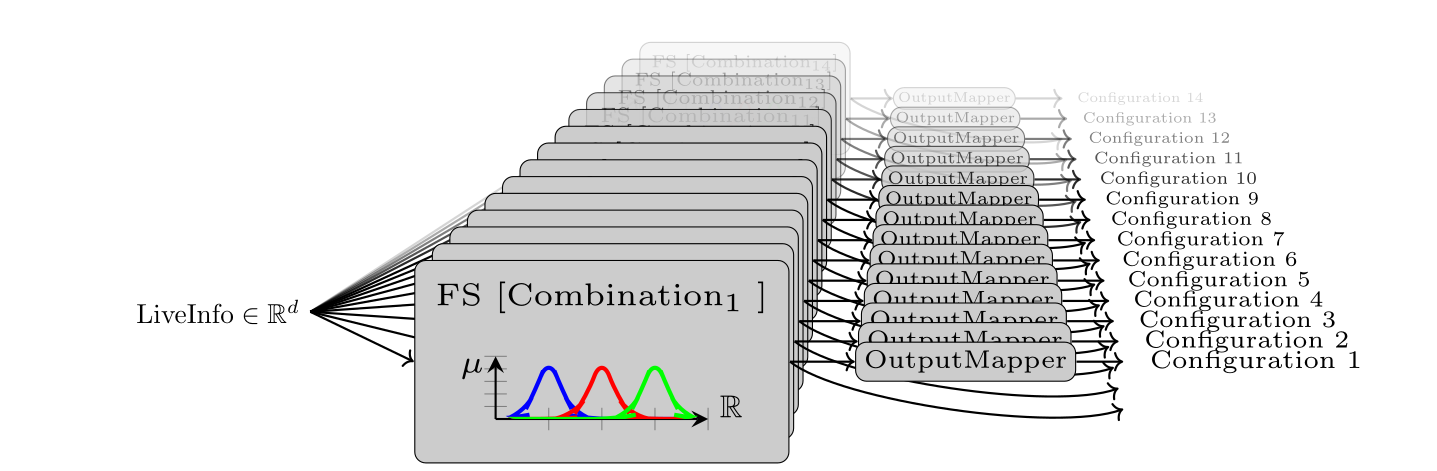
\includegraphics[width=1\textwidth]{figures/suitability-approach.png}
	\end{figure}
\end{frame}


\begin{frame}
	\frametitle{Approach 2: Suitability Tuning}
	\begin{itemize}
		\item Each configuration has a separate suitability variable
		\item Example rule:
		      \begin{itemize}
			      \item
			            \textbf{IF} threadCount is \textit{high} \textbf{AND} avgParticlesPerCell is \textit{low}\\ \qquad \textbf{THEN} suitability\_LinkedCells\_AoS\_lc\_c18\_disabled is \textit{bad}
			      \item Where \textit{high, low, bad} are appropriate linguistic terms
		      \end{itemize}
	\end{itemize}

	\begin{figure}
		\centering
		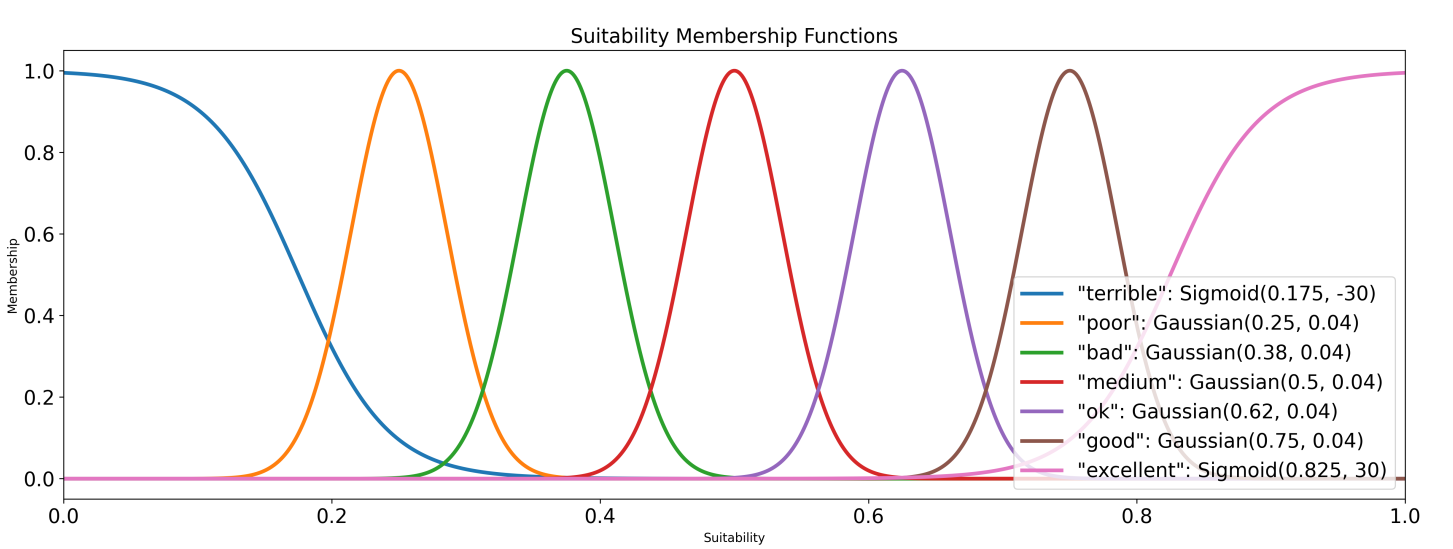
\includegraphics[width=1\textwidth]{figures/suitability-linguistic-variable.png}
	\end{figure}

\end{frame}


\section{Data-Driven Rule Extraction}
\begin{frame}
	\frametitle{Data-Driven Rule Extraction}
	\begin{itemize}
		\item Creating the Fuzy Rules is hard
		      \begin{itemize}
			      \item Expert Knowledge is required
			      \item Formalization of knowledge is difficult
			      \item Potentially many rules required
		      \end{itemize}
		\item Use Machine Learning to extract rules from data
		\item Decision Tree $\rightarrow$ Fuzzy Decision Tree $\rightarrow$ Fuzzy Rules {\footnotesize \cite{CROCKETT20062809}}
		\item Does not require expert knowledge
		\item Human experts can still validate the rules
	\end{itemize}
\end{frame}

\begin{frame}
	\frametitle{Conversion Process}

\end{frame}

\section{Comparison and Evaluation}
\begin{frame}
	\frametitle{Comparison and Evaluation}
	\begin{itemize}
		\item Exploding Liquid Benchmark
		\item Spinodal Decomposition MPI
		\item Further Analysis
	\end{itemize}
\end{frame}

\section{Future Work}
\begin{frame}
	\frametitle{Future Work}
	\begin{itemize}
		\item Dynamic Rule Generation
		\item Improving Tuning Strategies
		\item Simplification of the Fuzzy System
	\end{itemize}
\end{frame}

\section{Conclusion}
\begin{frame}
	\frametitle{Conclusion}
	\begin{itemize}
		\item Summary of Findings
		\item Impact
		\item Final Thoughts
	\end{itemize}
\end{frame}

\begin{frame}[allowframebreaks]
	\frametitle{References}
	\bibliographystyle{apalike}
	\bibliography{literature}
\end{frame}

\end{document}
